\documentclass[11pt,letterpaper]{article}

%\usepackage{times}
%\usepackage{epsfig}
\usepackage{graphicx}
%\usepackage{amsmath}
%\usepackage{amssymb}
\usepackage{hyperref}
\usepackage{tabularx}
\usepackage[left=1in, right=1in, top=1in, bottom=1in]{geometry}
\usepackage{titling}
\usepackage{setspace}
\usepackage{sectsty}
\usepackage{tabto}
\graphicspath{{./final_project_phase_2_files/}} % adds the assets directory to the path, throw your images there
\usepackage{fancyhdr}
\pagestyle{fancy}
\fancyhf{}
\fancyheadoffset{0cm}
\renewcommand{\headrulewidth}{0pt} 
\renewcommand{\footrulewidth}{0pt}
\fancyhead[R]{\thepage}
\fancypagestyle{plain}{%
  \fancyhf{}%
  \fancyhead[R]{\thepage}%
}

\usepackage{cite}
\usepackage[sectionbib]{natbib}
\renewcommand{\refname}{}

\usepackage{rotating}
\usepackage{dirtree}

\begin{document}
\fontfamily{ptm}\selectfont
\sectionfont{\fontsize{12}{12}\fontfamily{ptm}\selectfont}
\doublespacing
%%%%%%%%%%%%%%%%%%%%%%%%%%%%%% TITLE %%%%%%%%%%%%%%%%%%%%%%%%%%%%%%%%%%%%%%
\setlength{\droptitle}{1in} 

\title{\large{AI AGENT-POWERED AUTOMATION FOR PELOTON FITNESS ECOSYSTEM: \\ DESIGN \& PROTOTYPE PHASE \\\vspace{1.2in}}}

\author{
Kevin Geidel \\
MSDS 442: AI Agent Design \& Development \\
Northwestern University \\
June 1, 2025 \\
}

\date{}
\maketitle
\thispagestyle{empty}	
\clearpage
\setcounter{page}{1}

%%%%%%%%%%%%%%%%%%%%%%%%%%%%%% PAGE 1 %%%%%%%%%%%%%%%%%%%%%%%%%%%%%%%%%%%%
\section*{Requirement 1: Directory structure and training data}
\tab There are a number of files involved in prototyping the Peloton automation AI agent.
A full breakdown of the project's code base can be found in figure \ref{fig:dirtree}. \texttt{Analysis.pdf} is this document. \texttt{requirements.txt} is a list of all the Python packages needed to run the agent. They can be installed using \texttt{pip} and a Python virtual environment manager (such as \texttt{pyenv}.) There are some instructions for cloning the repository in order to run the agent on your local machine in the \texttt{README}.

\begin{figure}[h!]
    \centering
    \begin{minipage}{0.9\linewidth}
    \dirtree{%
        .1 msds442/.
        .2 Analysis.pdf.
        .2 requirements.txt.
        .2 README.md.
        .2 peloton/.
        .3 src/.
        .4 ai\_agent\_test\_data.json.
        .4 peloton\_data\_chatgpt\_raw\_responses.ipynb.
        .3 \_\_init\_\_.py.
        .3 agents.py.
        .3 Phase\_2\_NOTEBOOK\_Geidel.ipynb.
    }
    \end{minipage}
    \caption{Directory structure for Peloton AI Agent}
    \label{fig:dirtree}
\end{figure}

Inside the \texttt{peloton/} directory we see the \texttt{src/} directory. This contains the agent data used for testing. 
The test data was generated (in phase 1) through a series of prompts to ChatGPT (\url{https://chatgpt.com/}). 
The prompts and raw outputs are stored in \texttt{peloton\_data\_chatgpt\_raw\_responses.ipynb}.
The generated test data covers the five AI agents (marketing, data science, membership \& fraud detection, orders and product recommendations.)
Each agent has test data that supports at least three specific user stories. The records are stored, in JSON format, in \texttt{ai\_agent\_test\_data.json}.
A sample of what these JSON objects look like can be seen in figure \ref{fig:test_data}

Back in the \texttt{peloton/} directory we see \texttt{\_\_init\_\_.py}. This file makes the \texttt{peloton/} directory recognizable as a Python module to the interpreter and allows us to import it as such. The actual \texttt{PelotonAgent} class is defined in \texttt{agents.py} and will be described in further detail below (requirement 3.) The Jupyter notebook file, \texttt{Phase\_2\_NOTEBOOK\_Geidel.ipynb}, is used for the demonstration. It simply imports the agent class, instantiates an instance, renders a graphic that depicts the LangGraph and invokes the agent.

\clearpage

\begin{figure}[h]
    \centering
      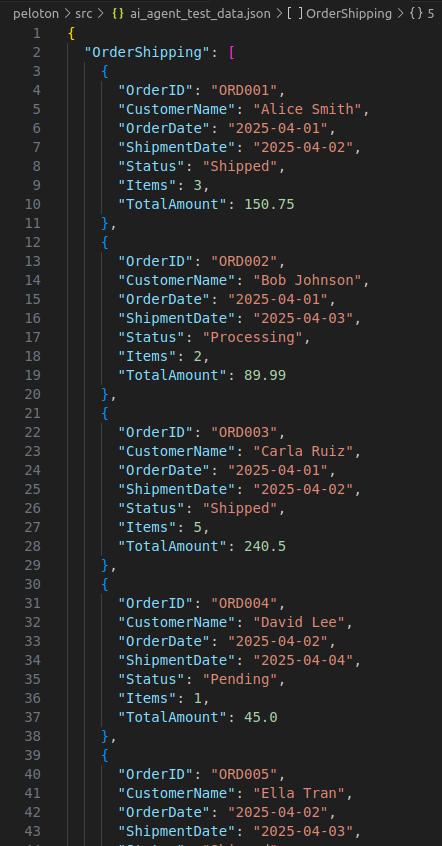
\includegraphics{test_data_json.png}
      \caption{A sample of the test data in JSON format.}
    \label{fig:test_data}
\end{figure}

\section*{Requirement 2: LangGraph architecture}
\tab The actual agent graph is created (using \texttt{LangGraph}) in the \texttt{build\_graph} method of the \texttt{PelotonAgent} class (see lines 116-143 in the attached listing.) The nodes and their respective functions are defined above this. Note the use of conditional edges to allow for agent choice and the inclusion of a \texttt{ToolNode} that houses the LangChain retriever. The result of integrating these agents into this workflow can be seen graphically in figure \ref{fig:graph}. Dotted lines indicate conditional edges.

\begin{figure}[h]
    \centering
      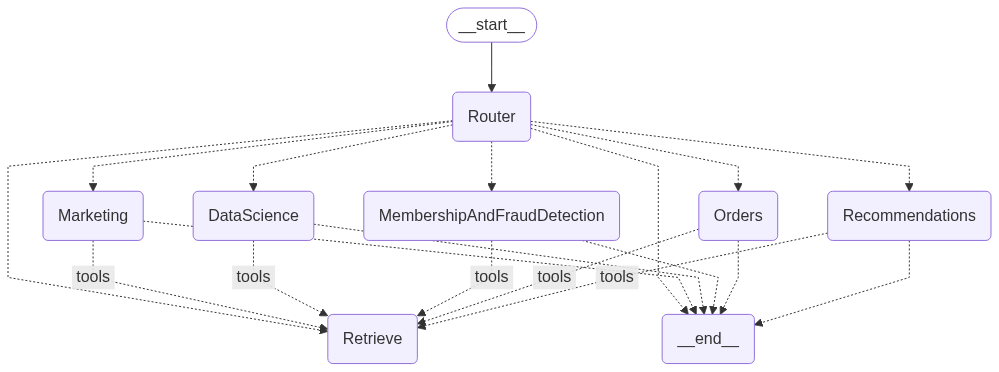
\includegraphics[width=1.0\linewidth]{graph.png}
      \caption{The Peloton agent architecture.}
    \label{fig:graph}
\end{figure}

\section*{Requirement 3: Implementation}
\tab Three area specific agents (plus the router agent) are implemented in this phase (marketing, data science and membership/fraud detection.)
In order to discuss their implementation we must examine the \texttt{PelotonAgent} class defined in \texttt{agents.py}. The contents of this file are included in the attached listing. \texttt{LangGraph} is a stateful machine and we give our state attributes in lines 47-52. Each node will track the current inquiry, the latest response, the node that referred the inquiry to the current node and the name of the next node to forward to. Messages are included to provide memory in the form of historical context. Upon instantiating an object of this class we create an LLM client, load the test data into LangChain documents and store these documents in a ChromaDb vector store (lines 61, 64 and 67 respectively.)
\texttt{load\_documents} and \texttt{populate\_vector\_store} and class methods defined below. There are several additional worker methods defined on the class that perform utility functions- mostly to abstract/DRY-out the code. The agent definitions themselves begin on line 201 with the \texttt{router\_agent}. The core function of the router is to classify the user's intent and set \texttt{next\_node} accordingly. 

The implemented agents share similar patterns. They are centered around a system prompt that defines their purpose and queries the LLM on behalf of the user. All messages, AI, System and Human are added to the messages list to maintain a memory of the conversation over multiple iterations.

\section*{Requirement 4: Working prototype}
\tab Three user stories (one for each of the implemented agents) were tested. All three agents are able to access their respective data from the store. The marketing agent was developed so that it might extract analyze the performance of ongoing marketing campaigns. The data science agent is able to derive insights from metrics in the data store. The membership agent can answer questions about potential fraudulent accounts. The following transcript of a session tried to demonstrate all of the implemented features: routing, accessing data, drawing insights and access to general knowledge from LLM training.

\begin{figure}[h]
    \centering
      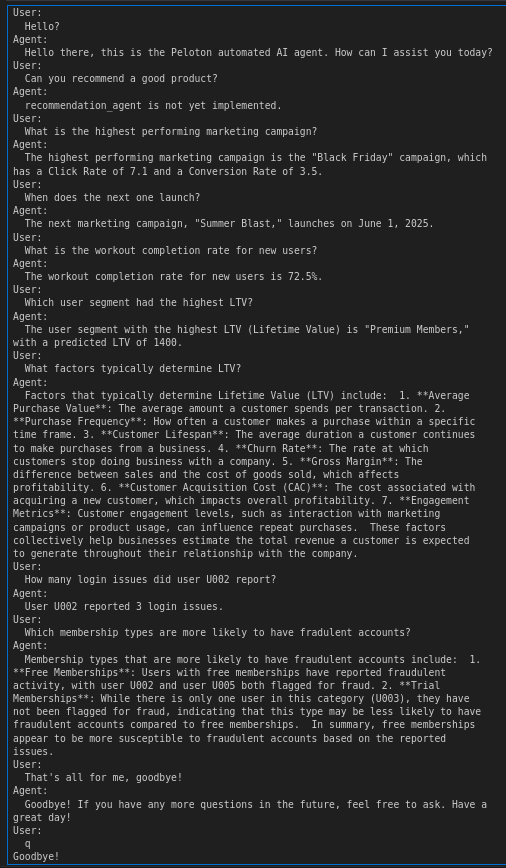
\includegraphics[height=1.0\textheight]{transcript.png}
      \caption{Example session that jogs three user stories and other features.}
    \label{fig:transcript}
\end{figure}

\end{document}